\chapter{Étude préliminaire et fonctionnelle}

\section{Introduction}
Ce chapitre a pour objectif de cadrer les besoins auxquels le projet \textbf{CertifEns} doit répondre, qu’ils soient liés aux fonctionnalités principales, aux contraintes techniques ou encore à l’expérience utilisateur. Il permet également de clarifier l’identité des différents acteurs, ainsi que leur rôle dans le système. Enfin, il détaille la logique de fonctionnement au travers de cas d’utilisation et de l’analyse des besoins qui guideront la conception technique.

\section{Étude des besoins}
Dans cette section, nous distinguons deux grandes catégories de besoins : fonctionnels, qui décrivent les services offerts par la plateforme, et non fonctionnels, qui concernent les performances, la fiabilité et la sécurité globale du système.

\subsection{Besoins fonctionnels}
Les besoins fonctionnels représentent les actions spécifiques que le système CertifEns doit être capable d'exécuter pour satisfaire les utilisateurs finaux.

\subsubsection{Liste des fonctionnalités principales}
L'application propose les services essentiels suivants :
\begin{itemize}
    \item \textbf{Gestion des Certifications :} Création et configuration de parcours certifiants avec suivi de progression.
    \item \textbf{Surveillance automatisée (AI Proctoring) :} Détection de fraudes en temps réel via YOLOv8 et analyse du regard avec MediaPipe.
    \item \textbf{Génération de contenu pédagogique par IA :} Création instantanée de quiz et de résumés à l'aide d'Ollama et de modèles LLM locaux.
    \item \textbf{Encadrement et Suivi :} Système de gestion de tâches pour un accompagnement personnalisé des apprenants.
    \item \textbf{Collaboration synchrone :} Module de visioconférence intégré pour les réunions et les sessions de supervision en direct.
\end{itemize}

\subsubsection{Scénarios d'utilisation concrets}
Pour illustrer la valeur ajoutée de CertifEns, voici trois scénarios métiers types impliquant chaque acteur du système :

\begin{enumerate}
    \item \textbf{Scénario Formateur (Productivité et Interaction) :} Le formateur orchestre un cycle de certification depuis son espace dédié. Après avoir automatisé la création des évaluations pédagogiques, il anime des sessions d'échange en direct pour approfondir les concepts avec ses étudiants. Il utilise ensuite les outils de suivi pour assigner des objectifs personnalisés et accompagner la progression de chaque apprenant de manière structurée.
    
    \item \textbf{Scénario Apprenant (Parcours et Réussite) :} L'apprenant suit son évolution via un tableau de bord centralisé. Il participe à des évaluations sécurisées garantissant l'intégrité de son parcours, reçoit des notifications pour ses échéances importantes, et accède en fin de cursus à ses résultats détaillés pour obtenir une certification officielle valorisant ses compétences.
    
    \item \textbf{Scénario Administrateur (Gestion et Gouvernance) :} L'administrateur assure le pilotage global de la plateforme. Il supervise les comptes des différents intervenants, structure l'offre pédagogique en regroupant les formations par thématiques, et analyse les indicateurs de performance globaux pour optimiser la qualité des parcours certifiants proposés par l'organisation.
\end{enumerate}

\subsection{Besoins non fonctionnels}
Ces besoins garantissent que le système fonctionne de manière optimale, sécurisée et évolutive.

\subsubsection{Contraintes de performance, de sécurité et de fiabilité}
\begin{itemize}
    \item \textbf{Performance :} L'analyse vidéo pour le proctoring doit s'effectuer en quasi-temps réel (latence inférieure à 200ms) pour garantir une détection efficace.
    \item \textbf{Sécurité :} L'accès aux portails est protégé par une authentification JWT (\textit{JSON Web Token}). Les données sensibles et les flux vidéo sont sécurisés pour respecter la confidentialité des examens.
    \item \textbf{Fiabilité :} Le système doit assurer une haute disponibilité des services de visioconférence et une persistance sans faille des résultats de certification.
\end{itemize}

\subsubsection{Implications sur le choix de l’architecture et de la technologie}
Ces contraintes de performance et d'intégrité ont dicté nos choix stratégiques :
\begin{itemize}
    \item \textbf{Architecture Microservices :} Adoption d'un découplage entre les services métiers (Admin, Formateur, Apprenant) pour assurer la scalabilité et isoler les briques d'IA très gourmandes en ressources.
    \item \textbf{Frameworks de développement :} 
    \begin{itemize}
        \item \textbf{Spring Boot :} Pour la robustesse des services back-end et la gestion sécurisée des données.
        \item \textbf{FastAPI :} Pour l'exposition haute performance des modèles d'intelligence artificielle en Python.
        \item \textbf{React.js :} Pour une interface utilisateur réactive, moderne et ergonomique.
    \end{itemize}
    \item \textbf{Technologies d'IA et Temps Réel :}
    \begin{itemize}
        \item \textbf{Ollama :} Pour l'exécution locale des modèles de langage (LLM), garantissant la confidentialité des données pédagogiques.
        \item \textbf{LiveKit :} Pour la gestion des flux vidéo et audio haute performance lors des sessions de visioconférence.
        \item \textbf{YOLOv8 et MediaPipe :} Pour une surveillance visuelle (Proctoring) précise et optimisée.
    \end{itemize}
    \item \textbf{Infrastructure et Persistance :}
    \begin{itemize}
        \item \textbf{Docker :} Pour simplifier le déploiement et garantir la cohérence de l'environnement technique à travers toutes les briques de la plateforme.
        \item \textbf{PostgreSQL :} Pour une gestion relationnelle fiable et performante des données de certification.
    \end{itemize}
\end{itemize}

\section{Identification des acteurs}
L'identification des acteurs consiste à définir les différents profils qui interagiront avec le système CertifEns, ainsi que leurs droits et responsabilités respectifs.

\begin{itemize}
    \item \textbf{Administrateur :} Il assure le pilotage global de la plateforme. Ses responsabilités incluent la gestion du cycle de vie des comptes utilisateurs (formateurs et apprenants), l'organisation des formations en cycles et en lots thématiques (\textit{Bundles}), ainsi que la surveillance des indicateurs de performance globaux via des outils d'analyse statistique.
    
    \item \textbf{Formateur :} Acteur central de la pédagogie, il est responsable de la création des contenus et de l'évaluation. Il utilise les outils d'automatisation pour générer des banques de questions, anime les sessions de visioconférence en direct pour le tutorat, et assure un suivi personnalisé via le module d'encadrement structuré. Il a également accès aux rapports de supervision des examens de ses étudiants.
    
    \item \textbf{Apprenant :} Utilisateur final du service d'apprentissage, il accède à son espace personnel pour suivre ses cours et remplir ses objectifs d'encadrement. Il participe aux évaluations surveillées par l'intelligence artificielle et peut, après validation de ses compétences, consulter ses résultats et récupérer ses certificats officiels.
\end{itemize}

\section{Cas d’utilisation et diagrammes}
Les cas d'utilisation (\textit{Use Cases}) permettent de formaliser les interactions entre les acteurs et le système CertifEns. Ils offrent une vision claire des fonctionnalités du point de vue de l'utilisateur final.

\subsection{Présentation des cas d'utilisation}
Chaque acteur interagit avec le système pour atteindre des objectifs spécifiques. Le diagramme de cas d'utilisation global (voir figure \ref{fig:use_case_global}) illustre cette répartition des responsabilités.

\begin{figure}[H]
    \centering
    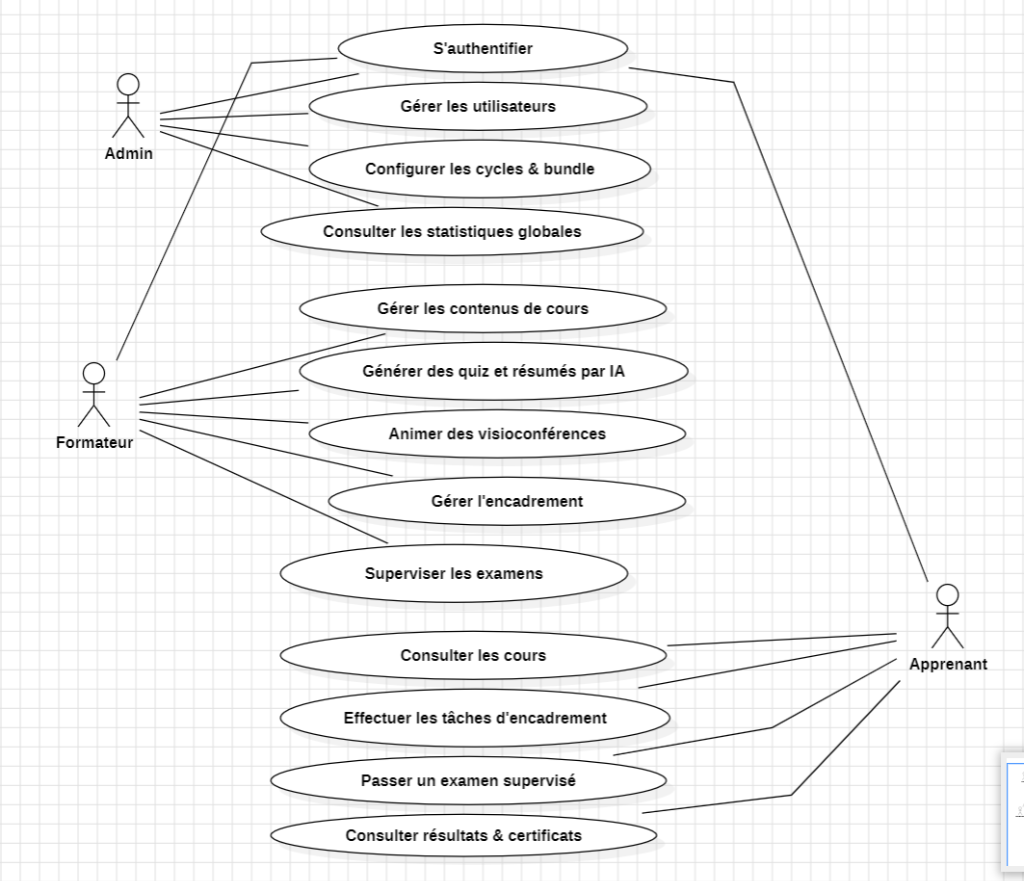
\includegraphics[width=0.85\linewidth]{figures/use_case_global.png}
    \caption{Diagramme de cas d'utilisation global de CertifEns.}
    \label{fig:use_case_global}
\end{figure}

Les cas d'utilisation principaux sont détaillés ci-dessous :
\begin{itemize}
    \item \textbf{Administrateur :}
    \begin{itemize}
        \item \textit{Gérer les utilisateurs :} Création, modification et suppression des comptes formateurs et apprenants.
        \item \textit{Organiser les formations :} Structuration des cours en cycles de certification et en bundles thématiques.
    \end{itemize}
    
    \item \textbf{Formateur :}
    \begin{itemize}
        \item \textit{Générer des évaluations par IA :} Utilisation du moteur LLM pour créer des quiz et des résumés.
        \item \textit{Animer des visioconférences :} Lancement de sessions de tutorat en direct.
        \item \textit{Superviser l'encadrement :} Suivi de la progression des tâches assignées aux apprenants.
    \end{itemize}
    
    \item \textbf{Apprenant :}
    \begin{itemize}
        \item \textit{Passer un examen supervisé :} Réalisation d'une évaluation sous surveillance IA.
        \item \textit{Suivre son parcours :} Consultation du tableau de bord de progression et des tâches d'encadrement.
        \item \textit{Consulter ses certificats :} Accès aux attestations de réussite validées.
    \end{itemize}
\end{itemize}

\subsection{Couverture des besoins fonctionnels}
Cette modélisation assure une couverture complète des besoins identifiés précédemment. Chaque fonctionnalité clé (surveillance, génération de contenu, encadrement) est directement reliée à un cas d'utilisation métier, garantissant ainsi la cohérence et la pertinence du système développé.

\section{Processus métier}
Le processus métier décrit l'enchaînement logique des opérations, depuis la préparation pédagogique jusqu'à la délivrance de la certification. Cette vision dynamique complète la vision statique des cas d'utilisation.

\subsection{Workflow global du système}
Le diagramme de processus présenté en figure \ref{fig:workflow_global} illustre le flux d'informations et les interactions entre les différentes briques technologiques de la plateforme.

\begin{figure}[H]
    \centering
    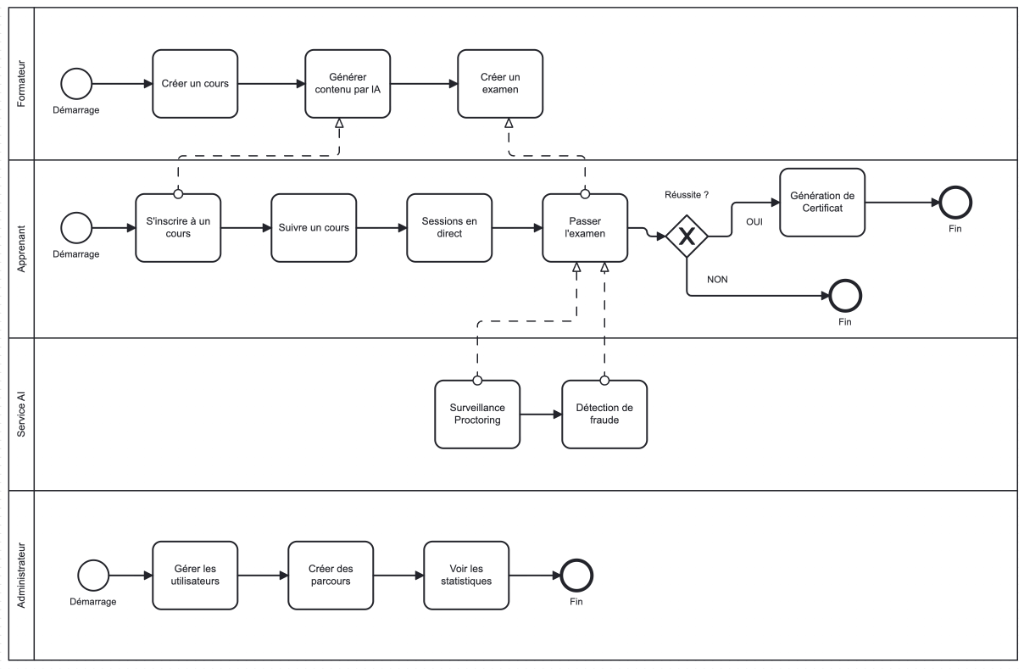
\includegraphics[width=0.85\linewidth]{figures/workflow_global.png}
    \caption{Diagramme de processus métier global (BPMN) de CertifEns.}
    \label{fig:workflow_global}
\end{figure}

\subsection{Validations et étapes-clés}
Le cycle de vie d'une certification repose sur plusieurs jalons critiques :
\begin{enumerate}
    \item \textbf{Gestion Administrative :} L'administrateur prépare l'écosystème en gérant les comptes et en structurant les cycles de formation.
    \item \textbf{Ingénierie Pédagogique :} Le formateur crée les contenus. L'intégration de l'IA permet une validation assistée via la génération de quiz et de résumés.
    \item \textbf{Parcours d'Apprentissage :} L'apprenant suit les modules, participe aux sessions d'échange en direct et effectue ses tâches d'encadrement.
    \item \textbf{Évaluation et Surveillance :} C'est l'étape de contrôle final. Le service de surveillance intelligente analyse les flux en temps réel pour garantir l'intégrité de l'examen. En cas de réussite, le certificat est généré automatiquement. En cas d'échec, le processus prend fin sans délivrance de titre.
\end{enumerate}

\section{Conclusion}
En conclusion, ce chapitre a permis de dresser un bilan synthétique de l'étude fonctionnelle et préliminaire de CertifEns. Nous avons défini une vision claire des fonctionnalités prévues, tout en précisant les rôles et responsabilités de chaque acteur (Administrateur, Formateur, Apprenant). Les contraintes majeures liées à la performance du temps réel et à la sécurité des évaluations ont été identifiées comme des piliers centraux de la conception.

Cette étude pose les bases nécessaires pour la suite de notre démarche. Le chapitre suivant sera consacré à l'\textbf{État de l'art}, où nous confronterons ces besoins avec les solutions et approches technologiques existantes, afin d'affiner la pertinence de nos choix techniques et de positionner CertifEns par rapport aux travaux préexistants dans le domaine de la certification intelligente.
